%\chapter*{\Large Anexos}
%\addcontentsline{toc}{chapter}{Anexos}
\appendix
\chapter{\Large Entorno de Virtualización}
    \begin{section}{Configuración del entorno de virtualización}
        Para el entorno de virtualización se utilizó VMWare ESXi \cite{vmware}, concretamente la suite vSphere HyperVisor v6.7.0 u3. Este sistema operativo basado en Unix permite gestionar los recursos de hardware disponibles, almacenar imágenes de distintos sistemas operativos y crear máquinas virtuales con estos últimos. Durante el proceso de creación de una máquina virtual, se selecciona el sistema operativo deseado y es posible asignar distintas cantidades de memoria principal, secundaria, cantidad de vCPU, número y tipo de enlaces de red, entre otros parámetros. \par
         \begin{figure}[H]
          \centering
           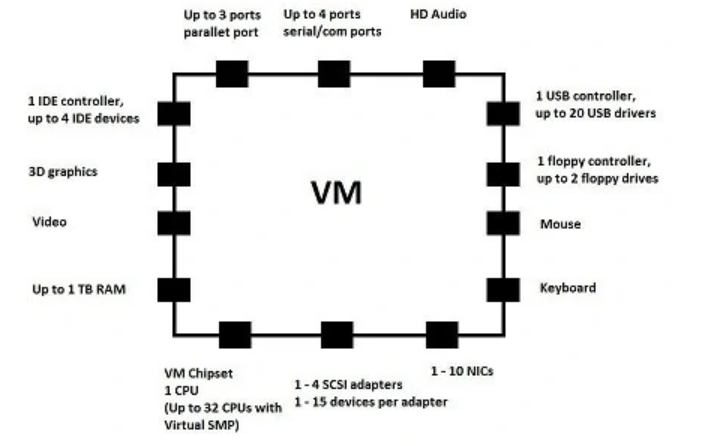
\includegraphics[width=0.7\textwidth]{./iteracion_1_imagenes/figura_34_diagrama_VM.png}
            \caption{ Diagrama de una máquina virtual desde el punto de vista de un HyperVisor\cite{vmware}}
            \label{fig:maquina_virtual}
        \end{figure}
        \end{section}
        
\chapter{\Large Configuración del sistema base}
\begin{section}{Introducción}
        Es posible instalar Security Onion en su versión 16.04 de dos maneras: mediante una ISO provista por los desarrolladores o bien mediante una serie de paquetes en una distribución Ubuntu \cite{ubuntu}. En este último caso será necesario contar con la distribución Ubuntu en su versión 16.04, ya que las distribuciones de Security Onion siguen a las distribuciones respectivas de Ubuntu. A partir del año 2020 se lanzaron nuevas versiones de Security Onion con soporte a otras distribuciones Linux: CentOS 7 y Ubuntu 18.04 y 20.04, aunque en el futuro se podrá desplegar en otros tipos de sistema Linux. Desde la versión 2.x de Security Onion en adelante, el sistema se despliega en contenedores.
        \end{section}
        \begin{section}{Instalación y configuración de Security Onion}
        Como se mencionó en la sección anterior, existen dos maneras de instalar esta versión de Security Onion: a partir de una imagen ISO o mediante paquetes. \par 
        En primer lugar se crearon dos máquinas virtuales sobre el hipervisor VMWare ESX(i), con los requisitos definidos en la sección \ref{seleccion_hw} para un nodo Master y Forward.\par
        En las maquinas virtuales se utilizo la ISO de Security Onion. La instalación se realizo mediante el asistente integrado que dispone la imagen del sistema operativo. Este asistente comenzo por configurar la interfaz de red como enlace de administración, como se ve en la Figura \ref{fig:figura_37_sonion_conf}. Se solicito ingresar parámetros para la configuración de IP estática o dinámica, servidor DNS, etc. \par
        \begin{figure}[H]
            \centering
            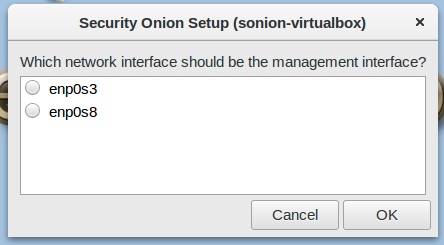
\includegraphics[width=0.5\textwidth]{./iteracion_1_imagenes/figura_37_sonion_conf.png}
            \caption{Elección de la interfaz de administración}
            \label{fig:figura_37_sonion_conf}
        \end{figure}
        \FloatBarrier
        En segundo lugar, el asistente preguntó si se deseaba configurar una interfaz para monitoreo. Este paso fue importante ya que si lo que se estaba desplegando era un nodo Master en una topología distribuida, habia que elegir la opción de no implementar una interfaz de monitoreo. Cuando tuvimos que desplegar un nodo Forward en una topología distribuida fue necesario seleccionar la opción para configurar una interfaz para monitorear tráfico de red. \par
        Luego de aceptar las modificaciones propuestas por el asistente, el sistema se reinició. Completado el reinicio, fue necesario volver a ejecutar el asistente de instalación, que nuevamente preguntó si se deseaba configurar las interfaces de red. Fue necesario seleccionar la opción de saltar este paso, tras lo cual el asistente preguntó el modo de despliegue del sistema: evaluación o producción, como se ve en la figura \ref{fig:figura_38_sonion_modo}
        \begin{figure}[H]
            \centering
            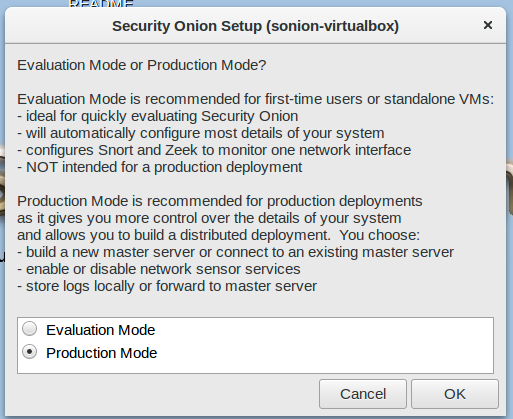
\includegraphics[width=0.7\textwidth]{./iteracion_1_imagenes/figura_38_sonion_modo.png}
            \caption{El asistente de instalación permitía elegir el modo de despliegue}
            \label{fig:figura_38_sonion_modo}
        \end{figure}
        \FloatBarrier
        %Seleccionado el modo de despliegue, se debió elegir entre un nuevo despliegue de Security Onion o agregar la instalación actual a un entorno existente, como se ve en la figura \ref{fig:figura_38_b_sonion_modo}. Elegida la primer opción, se creó automáticamente un nodo Master, mientras que la opción restante configuraba un nodo Forward si hubiese sido seleccionada. \par
        Seleccionado el modo de despliegue, se debió elegir entre la creación de un nodo Máster o añadir un nuevo nodo Forward a una topología preexistente, como se ve en la figura \ref{fig:figura_38_b_sonion_modo}. Elegida la primer opción, se creó automáticamente un nodo Master, mientras que la opción restante configuraba un nodo Forward si hubiese sido seleccionada. \par
        \begin{figure}[H]
            \centering
            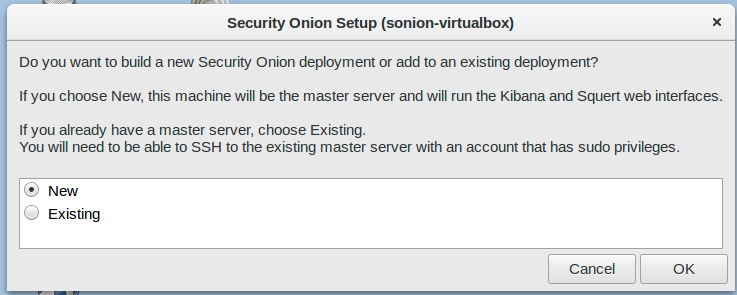
\includegraphics[width=0.7\textwidth]{./iteracion_1_imagenes/figura_38_b_sonion_modo.png}
            \caption{Elección entre la creación de un nodo Máster o añadir un nuevo nodo Forward a una topología preexistente}
            \label{fig:figura_38_b_sonion_modo}
        \end{figure}
        El asistente solicito el ingreso de datos para crear una cuenta de usuario y la elección de una configuración automática o manual para el resto de las opciones: persistencia de la base de datos mysql (por defecto 30 días), número de días de respaldo en caso de falla (por defecto 7 dias), selección de conjunto de reglas de detección (Emerging Threats Open o versiones de pago), motor de IDS (suricata o snort), habilitación de los sensores IDS (no recomendado para el nodo Master), SALT y activar o no la pila Elastic. Por último se debió seleccionar el almacenamiento de los logs: localmente o en un nodo de almacenamiento, así como el tamaño límite.\par
        Posteriormente se desplegó un nodo Forward. Las configuraciones ofrecidas por el asistente fueron muy similares a las descritas para el nodo Master. Los cambios que se requirieron fueron los datos relacionados a la configuración de red del enlace al nodo Master, por lo que fue necesario que previamente exista este nodo. Finalmente, fue necesario habilitar la conexión ssh e ingresar las credenciales del nodo Master, para la comunicación mediante un autotunel ssh entre ambos nodos.\par
        Con el fin de realizar pruebas iniciales del sistema, se eligió el despliegue mediante una ISO. Posteriormente, cuando se comprobó el funcionamiento de la mayoría de sus componentes, se desplegó el sistema mediante paquetes de la distribución 16.04 de Security Onion. Esta decisión se tomo debido a una solicitud de la organización, ya que esta contaba con maquinas virtuales configuradas con Ubuntu 16.04. \par
        Se dispuso de un sistema operativo Ubuntu Server 16.04 con la particularidad de tener dos discos montados: el principal para el sistema operativo y el secundario para los datos recolectados en un directorio \textbf{/nsm}. En el caso de un servidor Master se almacenaron índices en este directorio. En el caso de un nodo Forward, en el directorio \textbf{/nsm} se resguardaron capturas de paquetes o logs. \par 
        Sin importar el método de instalación, al finalizar el proceso, las configuraciones que se mencionaron anteriormente también se pudieron llevar a cabo mediante el comando \textit{sosetup -f $\sim$/sosetup.conf}. Esta instrucción ejecuta un programa que lee las configuraciones previamente guardadas en un archivo.\par
        Con el objetivo de cumplir uno de los requerimientos no funcionales del proyecto, que implica la automatización del despliegue (instalación y configuración) del sistema, se utilizó una herramienta de administración automatizada de servidores llamada Ansible en su versión 2.8.4 para la cual se desarrollaron scripts YAML conteniendo la secuencia de instalación de los paquetes, configuraciones, rol del nodo (Forward o Master) y librerías requeridas para el apropiado funcionamiento del sistema.\par
        \end{section}
        
        \begin{section}{Instalación y configuración de TheHive - Cortex}
        Para la instalación del gestor de incidentes, que tiene como componentes a  TheHive y Cortex, se utilizó  el sistema operativo Debian 10. En primer lugar se instaló TheHive, para ello fue necesario realizar la instalación previa de los componentes necesarios como las librerías de Java 8, Python (versiones 2.7 y 3.6) y Elasticsearch; este último requirió una configuración en su archivo elasticsearch.yaml, como se ve en la Figura \ref{fig:figura_39_thehive_conf}:
        
        \begin{figure}[H]
            \centering
            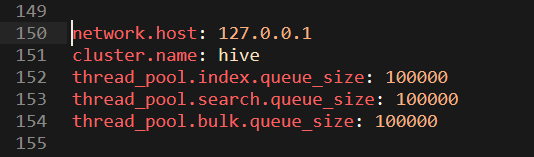
\includegraphics[width=0.7\textwidth]{./iteracion_1_imagenes/figura_39_thehive_conf_elastic.png}
            \caption{Configuración añadida a elasticsearch.yaml para la instalación de TheHive}
            \label{fig:figura_39_thehive_conf}
        \end{figure}
        Las modificaciones realizadas a este archivo fueron:
        \begin{itemize}
            \item network.host: dirección IP del servidor que contiene Elasticsearch, en este caso es el mismo por lo que se indico la dirección local.
            \item cluster.name: nombre del cluster en el que se desplegó Elasticsearch.
            \item Thread\_pool.index.queue\_size: tamaño de la cola de índices.
            \item Thread\_pool.search.queue\_size: tamaño de la cola para operaciones de búsqueda pendientes.
            \item Thread\_pool.bulk.queue\_size: tamaño de la cola de operaciones de escritura pendientes para un documento.
        \end{itemize}
        \par
        Finalmente, los últimos pasos para la instalación de TheHive consistieron en habilitar e iniciar el servicio de elasticsearch, agregar el repositorio que contiene los paquetes de TheHive, instalarlo y luego habilitar el servicio para poder iniciarlo. \par
        En cuanto a Cortex, el proceso fue similar al anteriormente descrito para TheHive, donde una vez descargados e instalados los paquetes de Cortex con su correspondiente secuencia de habilitación e inicio; se procedió a descargar del repositorio los responders y analyzers respectivos. Por último, se modificó el archivo de configuración de Cortex para indicar la ubicación del directorio que contiene los responders y analyzers mencionados anteriormente. \par
        Posteriormente se actualizó la base de datos elasticsearch mediante la GUI web de Cortex, se creó un superusuario y luego las organizaciones donde se administraron usuarios comunes y analyzers; fue necesario crear un usuario con el rol de administrador de organizaciones. Las organizaciones tuvieron habilitados y configurados determinados responders y analyzers según fue necesario. \par
        El último paso del proceso consistio en comunicar TheHive y Cortex entre sí. Para ello se generó una API key en Cortex que fue usada como parte de las modificaciones necesarias al archivo application.conf de TheHive. Las modificaciones completas que se realizaron al mencionado archivo se pueden apreciar en la Figura \ref{fig:figura_40_thehive_cortex_conf}:\par
        
        \begin{figure}[H]
            \centering
            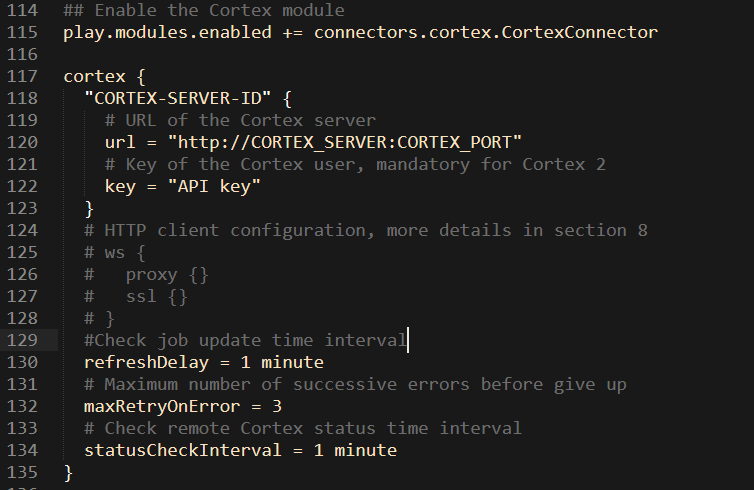
\includegraphics[width=0.7\textwidth]{./iteracion_1_imagenes/figura_40_thehive_cortex_conf.png}
            \caption{Modificación al archivo application.conf de TheHive para la comunicación con Cortex}
            \label{fig:figura_40_thehive_cortex_conf}
        \end{figure}
        Los campos modificados que se pueden observar son:
        \begin{itemize}
            \item play.modules.enabled: habilita el módulo de Cortex
            \item url: especifica la dirección url del servidor de Cortex
            \item key: Es API key del usuario de Cortex.
            \item refreshDelay: periodo de tiempo de comprobación de casos generados por TheHive
            \item maxRetryOnError: número máximo de intentos de recuperación de un error
            \item statusCheckInterval: periodo de tiempo de comprobación del estado de Cortex
        \end{itemize}
        \end{section}
    
\chapter{\Larger Configuracion de ElastAlert}
Se escribieron archivos de configuración para cada tipo de evento, de manera tal que las reglas que disparan cada alerta lo hagan según el comportamiento y naturaleza del incidente. En las figuras \ref{fig:iter2_1_codigo} a \ref{fig:iter2_4_codigo} se observa el código desarrollado para el envío de alertas en caso de producirse un reconocimiento y escaneo de puertos. Las figuras corresponden al mismo archivo de configuración, pero cada una muestra una parte del código para facilitar la explicación del mismo.\par
    En la Figura \ref{fig:iter2_1_codigo} se muestra la primer parte del código de configuración de una regla:
    \begin{itemize}
        \item \textit{es\_host}: el nombre del host de la base de datos elasticsearch.
        \item \textit{es\_port}: el número de puerto del host de elasticsearch mediante el cual ElastAlert se contactara con la base de datos.
        \item \textit{name}: nombre de la regla. Debe ser único.
        \item \textit{type}: especifica el tipo de regla. En este caso es del tipo “frecuency”, que determina que esta regla se activará si al menos se produce cierto número de eventos en determinado intervalo de tiempo.
        \item \textit{num\_events}: especifica la cantidad de eventos necesarios para activar este tipo de regla.
        \item \textit{timeframe}: determina el marco temporal necesario para este tipo de reglas. Tiene un sub parámetro que especifica la unidad temporal y la cantidad de estas. En este caso optamos por un marco temporal de un (1) minuto.
    \end{itemize}
    \begin{figure}[H]
    \centering
        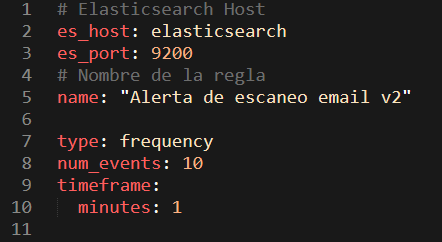
\includegraphics[width=0.7\textwidth]{./iteracion_2_imagenes/3-codigoAlerta-1.png}
        \caption{Primera parte del código de configuración de una regla}
        \label{fig:iter2_1_codigo}
    \end{figure}
    \FloatBarrier
    En la Figura \ref{fig:iter2_2_codigo} se muestran los campos implicados en la consulta a elasticsearch:
    \begin{itemize}
        \item \textit{index}: es el índice a consultar
        \item \textit{use\_strftime\_index}: es una variable booleana que, en el caso de ser verdadera, da formato al índice utilizando “\textit{datetime\_strftime}” para cada consulta. Este último método de Python crea un string representando el tiempo en un formato específico. Se utiliza en el caso de que la consulta realizada incluya varios días, con lo que los índices se concatenan utilizando “;” permitiendo una búsqueda más eficiente.
        \item \textit{filter}: determina los filtros de elasticsearch utilizados para la consulta. Utiliza los subparametros “term”  y “category” para indicar la clave a buscar. En este caso utilizamos “category: scan” para filtrar todos los eventos que pertenezcan a la categoría del reconocimiento de puertos.
        \item \textit{query\_term}: permite agrupar las consultas, en este caso agrupamos las alertas resultantes por direcciones IP de origen y destino, así como todos los eventos que tengan el campo “alert”.
        \item \textit{realert}: ignora las alertas repetidas en un cierto periodo de tiempo. En la práctica esto permitió evitar saturar con notificaciones a los responsables de los activos afectados, ya que el reconocimiento de puertos es un incidente extremadamente común y periódico, produciéndose muchas veces por día.
    \end{itemize}
    \begin{figure}[H]
    \centering
        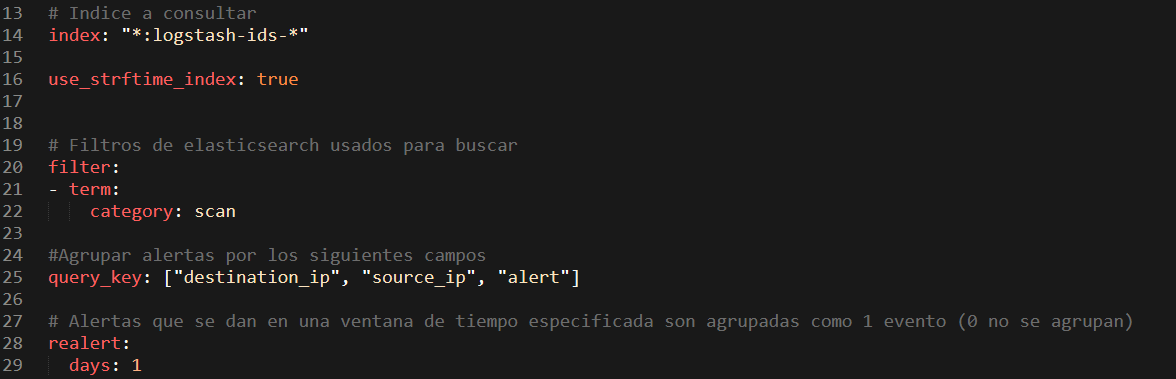
\includegraphics[width=1\textwidth]{./iteracion_2_imagenes/4-codigoAlerta2.png}
        \caption{Segunda parte del código de configuración de una regla}
        \label{fig:iter2_2_codigo}
    \end{figure}
    \FloatBarrier
    En la Figura \ref{fig:iter2_3_codigo} se observan los campos utilizados para armar el cuerpo del mensaje y el asunto:
    \begin{itemize}
        \item \textit{doc\_type}: especifica el tipo de documento a consultar en elasticsearch.
        \item \textit{alert\_subject}: permite personalizar el mensaje de una alerta agregando un pequeño resumen. En este proyecto lo utilizamos en todas las reglas, para que el “asunto” del correo electrónico contenga un mensaje de “Alerta: tipo-de-alerta”. En este caso el argumento ({0}) que figura es el primer campo (tipo de alerta) del objeto JSON que contiene la información del incidente.
        \item \textit{alert\_subject\_args}: contiene el nombre del campo que será utilizado por \textit{alert\_subject}
        \item \textit{alert\_text}: contiene el mensaje de la notificación, se decidió presentar en una lista los parámetros más importantes de los incidentes. Estos incluyen el nombre de la alerta (que también está en el asunto del correo), timestamp indicando la fecha y hora de la detección del incidente, dirección IP de destino, el puerto de destino, dirección IP y puerto de origen, la interfaz del sensor que realizó la detección, información sobre la firma del incidente y un link para verlo en kibana.
        \item \textit{alert\_text\_type}: especifica el formato del texto de la alerta, en este caso optamos por utilizar la sintaxis de formato standard de Python.
        \item \textit{alert\_text\_args}: contiene los nombres de los campos cuyos valores serán utilizados para el contenido del mensaje.
    \end{itemize}
    \begin{figure}[H]
    \centering
        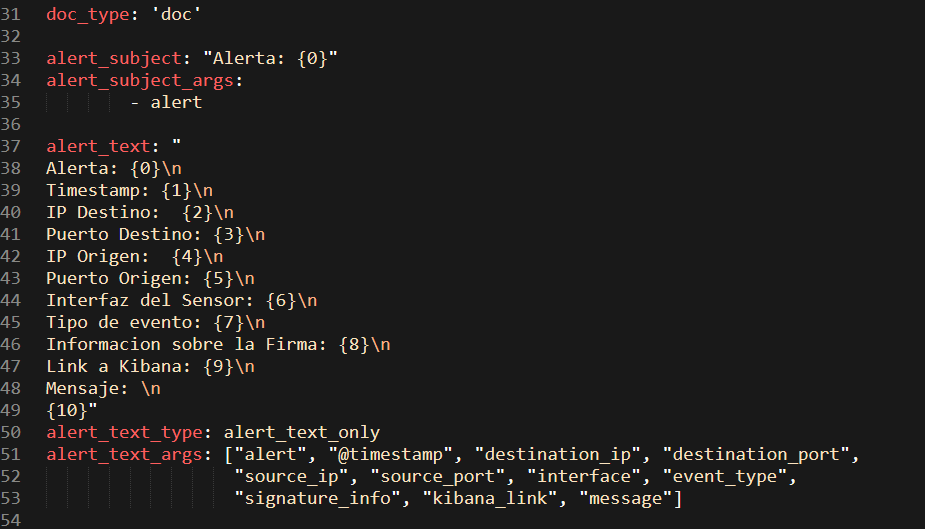
\includegraphics[width=1\textwidth]{./iteracion_2_imagenes/5-codigoAlerta3.png}
        \caption{Tercera parte del código de configuración de una regla}
        \label{fig:iter2_3_codigo}
    \end{figure}
    \FloatBarrier
    En la Figura \ref{fig:iter2_4_codigo} se observan los campos correspondientes al envío de la notificación:
    \begin{itemize}
        \item \textit{alert}: determina el tipo de alerta implementada, es decir, el método de envío. ElastAlert puede enviar mensajes y notificaciones por varios medios que incluyen el correo electrónico, servicios y aplicaciones, como Telegram, JIRA, entre otros. En este proyecto se decidió utilizar el correo electrónico de la organización como medio de notificación de alertas.
        \item \textit{email}: campo que contiene el correo electrónico de destino. Puede ser una dirección o una lista de direcciones de correos.
        \item \textit{from\_addr}: este campo contiene el correo electrónico remitente que ElastAlert utilizará para enviar las notificaciones.
        \item \textit{smtp\_host}: servidor SMTP del correo utilizado para enviar las notificaciones.
        \item \textit{smtp\_port}: puerto utilizado por el servidor SMTP.
        \item \textit{generate\_kibana\_link}: variable booleana que de estar activada genera un tablero temporal de Kibana y un link para acceder a el.
        \item \textit{use\_kibana4\_dashboard}: link hacia un tablero de Kibana (versión 4).
    \end{itemize}
    \begin{figure}[H]
    \centering
        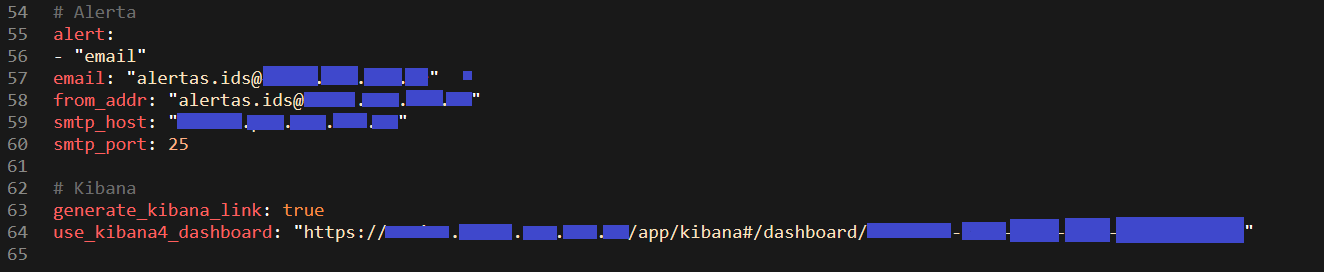
\includegraphics[width=1\textwidth]{./iteracion_2_imagenes/6-codigoAlerta4.png}
        \caption{Cuarta parte del código de configuración de una regla}
        \label{fig:iter2_4_codigo}
    \end{figure}
    \FloatBarrier
    
\chapter{Modificación de un filtro de Logstash}
El proceso de creación de este filtro consistió en copiar el archivo de configuración de Filebeat: \textit{9500\_output\_beats\_custom.conf} que se encuentra en el directorio mencionado anteriormente. El archivo fue copiado a la carpeta \textit{/etc/logstash/custom}, donde fue modificado para crear el filtro con Grok. Este fue creado teniendo en cuenta el cuerpo de los mensajes provenientes del archivo de logs analizado, dado que se conocían los campos de interés que contenían los logs y que por lo tanto se deseaba extraer. Una vez finalizada la modificación del archivo, se reinicio el servicio de Logstash y se comprobó que el archivo \textit{logstash.log} para verificar que no hubiera errores.\par


    


 
  

